\documentclass[11pt, a4paper]{article}
%\usepackage{proj1}
\usepackage{natbib}
\usepackage{fancyhdr}  
\usepackage{subcaption}
\usepackage{caption}
\usepackage{graphicx}
\usepackage{numprint}
\usepackage{multirow}
\linespread{1.25} 
\setlength{\parindent}{0cm}
\graphicspath{{Images/}}
\usepackage{hyperref}
\usepackage{amsmath}
\usepackage{amsfonts}
\usepackage{amssymb}
\usepackage{amsthm}
\usepackage{mathtools}
\usepackage{commath}
\usepackage{bbm}

%\usepackage[sc,osf]{mathpazo}
\usepackage{subcaption}
\usepackage[a4paper, top=1in, left=1.0in, right=1.0in, bottom=1in, includehead, includefoot]{geometry} %Usually have top as 1in

\usepackage{listings}
\usepackage{color} %red, green, blue, yellow, cyan, magenta, black, white
\definecolor{mygreen}{RGB}{28,172,0} % color values Red, Green, Blue
\definecolor{mylilas}{RGB}{170,55,241}


\hypersetup{colorlinks,linkcolor={black},citecolor={blue},urlcolor={black}}
\usepackage{color}
\urlstyle{same}


\theoremstyle{definition}
\newtheorem{definition}{Definition}[section]

%\newcommand{\Sta}{\rho}
\newcommand{\Adj}{p}
\newcommand{\adj}{q}
%\newcommand{\Con}{u}
\newcommand{\Sta}{\rho}
\newcommand{\Stav}{\mathbf{v}}
\newcommand{\Adja}{\mathbf{p}}
\newcommand{\Adjb}{q}
\newcommand{\Adjc}{{p}_{\partial \Sigma}}
\newcommand{\Con}{\mathbf{f}}
\newcommand{\nor}{\mathbf{n}}




\pagenumbering{gobble}
\begin{document}
	\section*{Report 03/09/2020}
	\section{Last Week}
	Implemented the dot product in shape and mulitshape.
	\section{Tests}
	Tested the forward problem and optimal control problem in different settings. It all seems to be working very well. 
	Forward Tests (Figure \ref{F0a}):
	\begin{itemize}
		\item Test 1: Compare computations on a box, with ADInf solution.
		\item Test 2: Compare on a box with AD Flow Neumann Exact solution.
		\item Test 3: Split box in MS code and compare to box in Box code using ADInf solution
		\item Test 3a: Same as 3 only checking that order of shapes don't matter.
		\item Test 4: Computing problem ADInf on wedge + quadrilateral
		\item Test 4a: Same as 4 only checking that order of shapes don't matter.
		\item ToyProblem 1: Computes no flux problem on two wedges and two quadrilaterals with constant 1 flow.
	\end{itemize} 
	Optimization Tests (Figure \ref{F0b}):
	\begin{itemize}
		\item Test 5: Comparing MS and Box code on a box with Neumann Flow Exact Problem
		\item Test 6: Split MS box in two parts and compare to box in Box code (same Exact solution)
		\item Test 7: Comparing on the box an interacting problem (problem one from paper)
		\item Test 8: Splitting MS box and comparing to Box code for interacting problem
	\end{itemize}
	\begin{figure}[h]
		\centering
		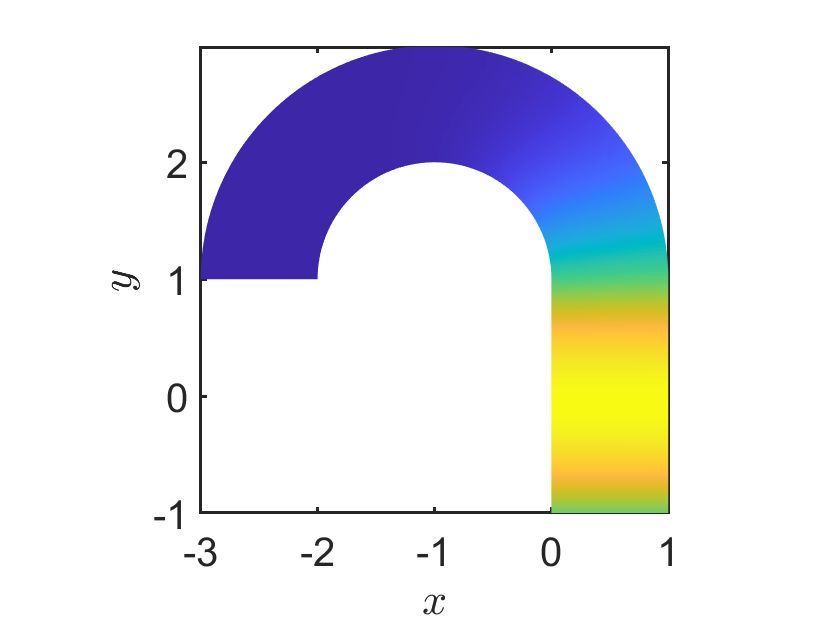
\includegraphics[scale=1]{T1.png}
		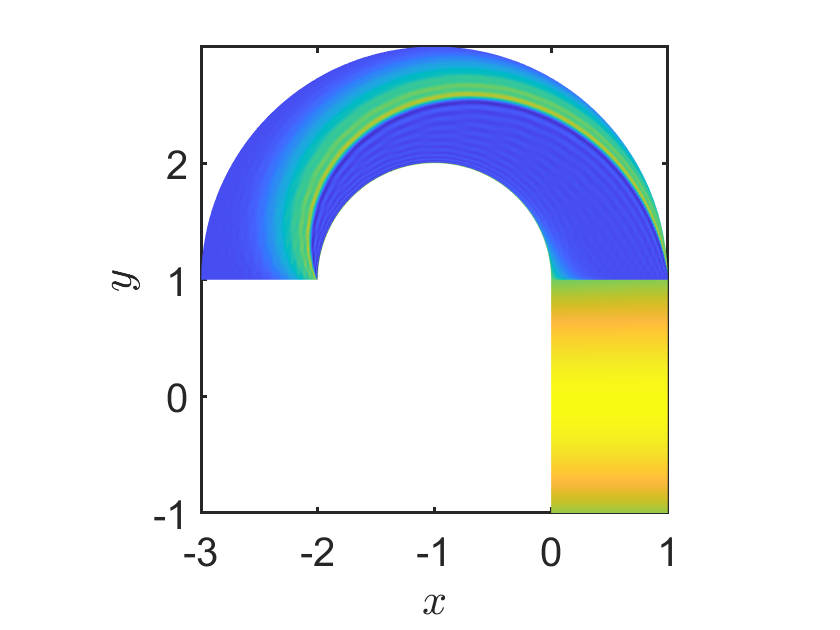
\includegraphics[scale=1]{T2.png}
		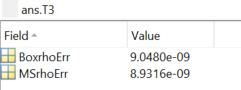
\includegraphics[scale=1]{T3.png}\\
		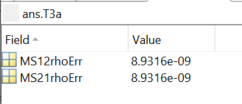
\includegraphics[scale=1]{T3a.png}
		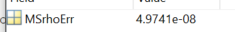
\includegraphics[scale=1]{T4.png}
		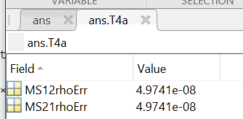
\includegraphics[scale=1]{T4a.png}
		\caption{Forward Test Solutions} 
		\label{F0a}
    \end{figure}
	\begin{figure}[h]
		\centering
		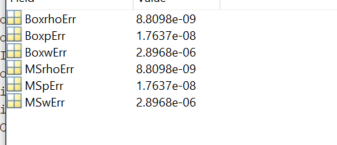
\includegraphics[scale=1]{T5.png}
		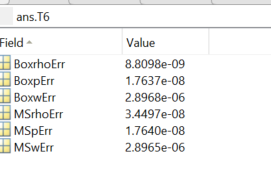
\includegraphics[scale=1]{T6.png}\\
		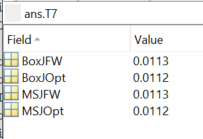
\includegraphics[scale=1]{T7.png}
		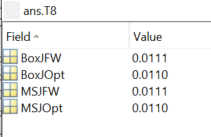
\includegraphics[scale=1]{T8.png}
		\caption{Optimization Test Solutions} 
		\label{F0b}
	\end{figure}
	
	\section{Comparing Matching Conditions in Forward problem}
	Compared with ADinf exact solution. Matching two boxes (vs full box)  and matching two wedges (vs full wedge). Both show that the results are the same regardless of the matching method.
	
	\begin{figure}[h]
		\centering
		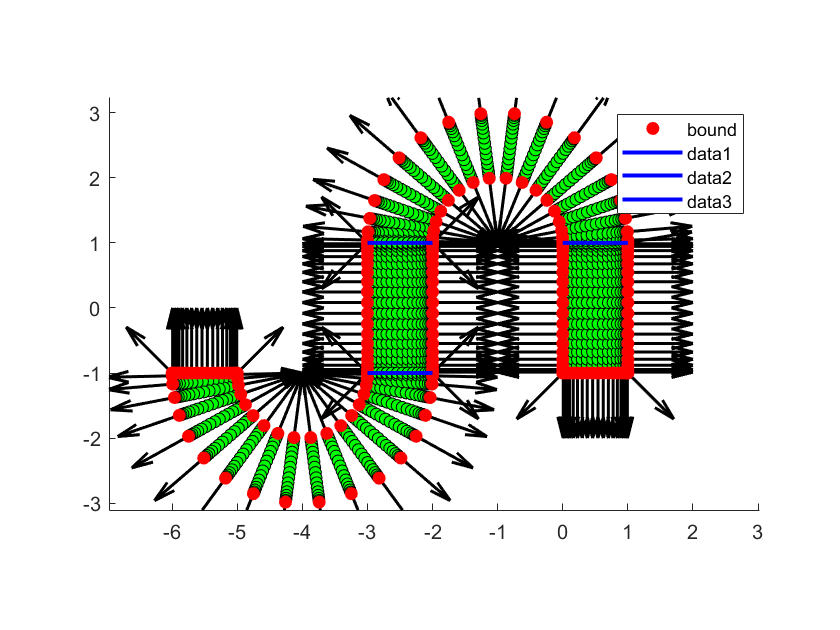
\includegraphics[scale=0.5]{dom1.png}
		\caption{Domain} 
		\label{FD1}
	\end{figure}
	Using the example with no flux and two wedges and two boxes (see Figure \ref{FD1}), the two matching methods are compared. The error in $\rho$ is $1.4292\times 10^{-10}$.
	
	
	\section{Finding distances between points that leave the domain}
    See Figure \ref{FI}. We decided that this is the way to do it. Still needs to be implemented.
    Aim: finding euclidean distance between each pair of points that crosses a boundary. This is to exclude those from the particle interaction, since those two particles then shouldn't interact.
		\begin{figure}[h]
		\centering
		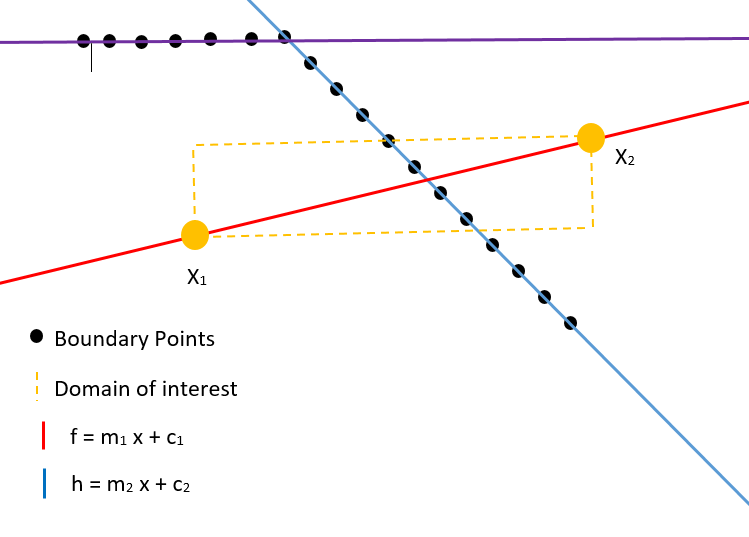
\includegraphics[scale=0.7]{Intersection.png}
		\caption{Intersection} 
		\label{FI}
    	\end{figure}
    
    
    
    \section{OCP on MultiShape}
    
    \subsection{Example 1}
    We choose the initial condition for $\rho$ to be $exp(-2((y1 - 0.5 )^2 + (y2 + 0.5)^2))$ and solve a forward problem with constant velocity of strength one, see Figure \ref{FTest1FW}.
    \begin{figure}[h]
    	\centering
    	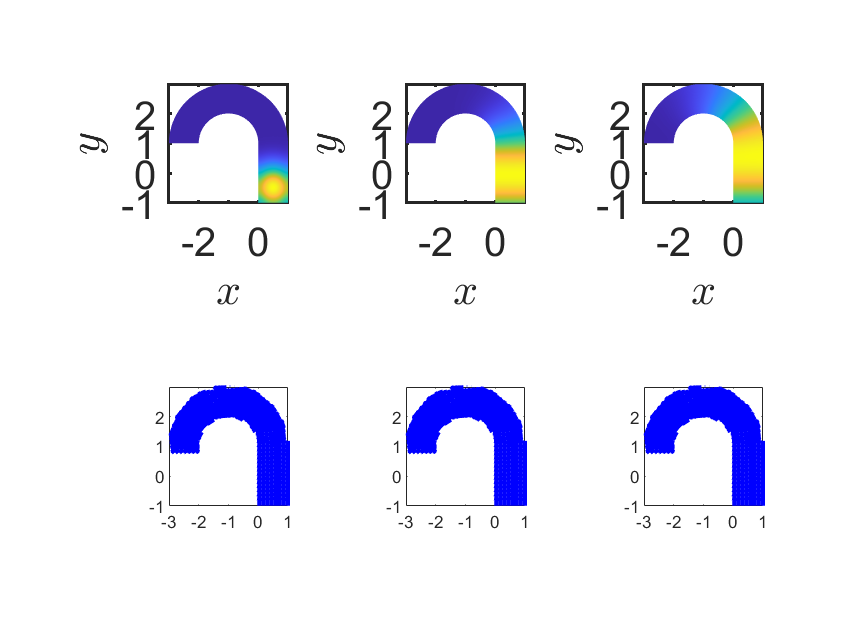
\includegraphics[scale=0.7]{Test10FW.png}
    	\caption{Test1 Forward $t =1, 10, 19, n = 20$} 
    	\label{FTest1FW}
    \end{figure}
    Then we use this forward solution as a target in the OCP, with initial velocity zero. We set $\beta = 10^{-3}$, we solve with tolerances $10^{-7}/ 10^{-3}$, because of time constraints, and $n = 20$, $N = 20$. The solution can be seen in Figure \ref{FTest1Opt}. As expected, the control follows the particle mass. It takes $452$ iterations, but the time it takes is $2 \times 10^4$. We get $J_{FW} = 0.0206$, $J_{Opt} = 0.0020$. 
    \begin{figure}[h]
    	\centering
    	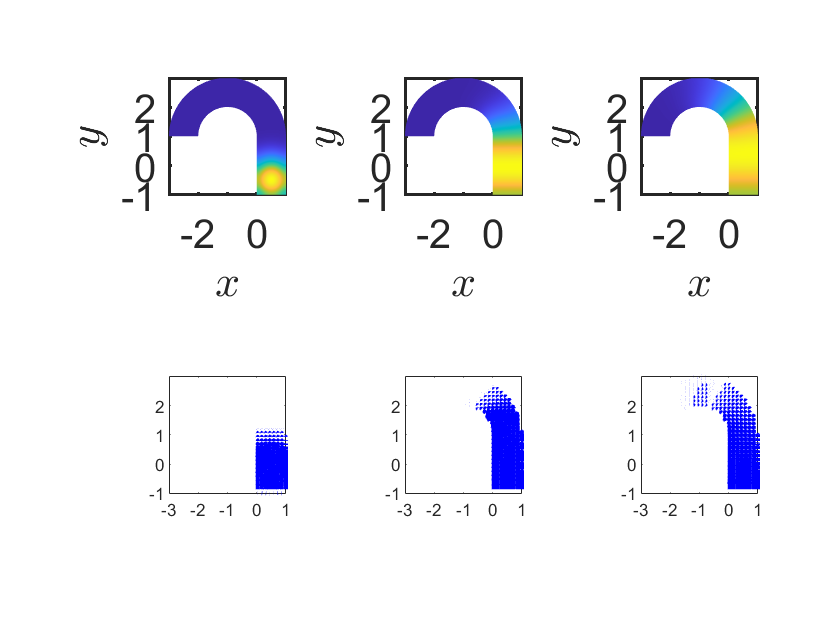
\includegraphics[scale=0.7]{Test10Opt.png}
    	\caption{Test1 Optimization $t =1, 10, 19, n = 20$} 
    	\label{FTest1Opt}
    \end{figure}
    We then choose $\kappa = -1$ and get $J_{FW} = 0.0251$, $J_{Opt} = 0.0020$, in $454$ iterations taking $ 1\times 10^4$ in time. We can see the results in Figures \ref{FTest1n1FW} and \ref{FTest1n1Opt}.
    \begin{figure}[h]
    	\centering
    	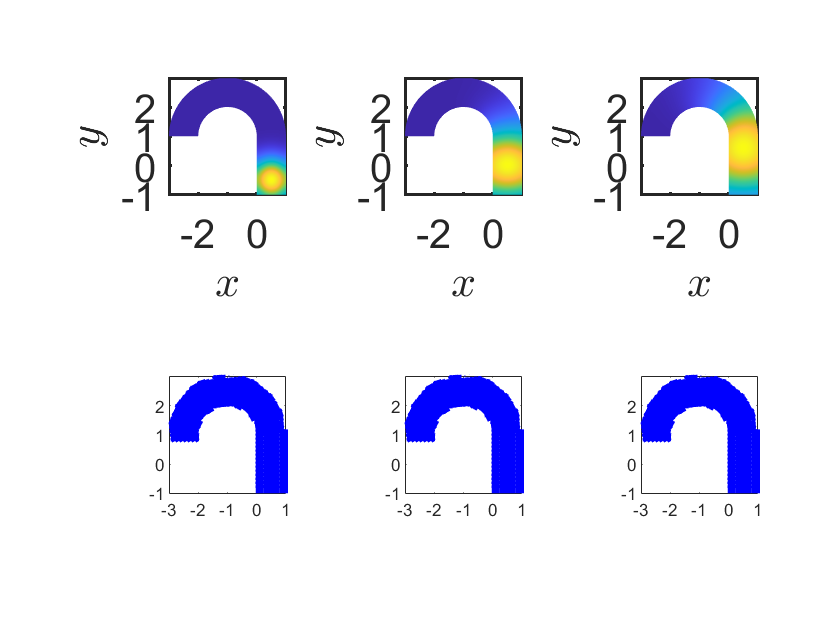
\includegraphics[scale=0.7]{Test10n1FW.png}
    	\caption{Test1 Forward $\kappa = -1$, $t =1, 10, 19, n = 20$} 
    	\label{FTest1n1FW}
    \end{figure}
    \begin{figure}[h]
    	\centering
    	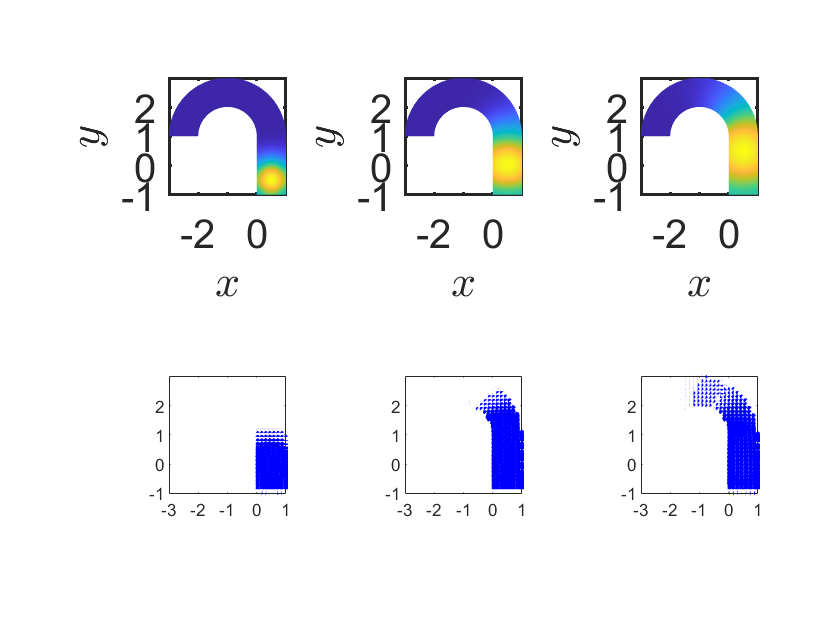
\includegraphics[scale=0.7]{Test10n1Opt.png}
    	\caption{Test1 Optimization $\kappa = -1$, $t =1, 10, 19, n = 20$} 
    	\label{FTest1n1Opt}
    \end{figure}
    We can do the same for $\kappa = 1$. We get $J_{FW} = 0.0176$, $J_{Opt} = 0.0020$, in $451$ iterations taking $ 1\times 10^4$ in time. We can see the results in Figures \ref{FTest11FW} and \ref{FTest11Opt}.
    \begin{figure}[h]
    	\centering
    	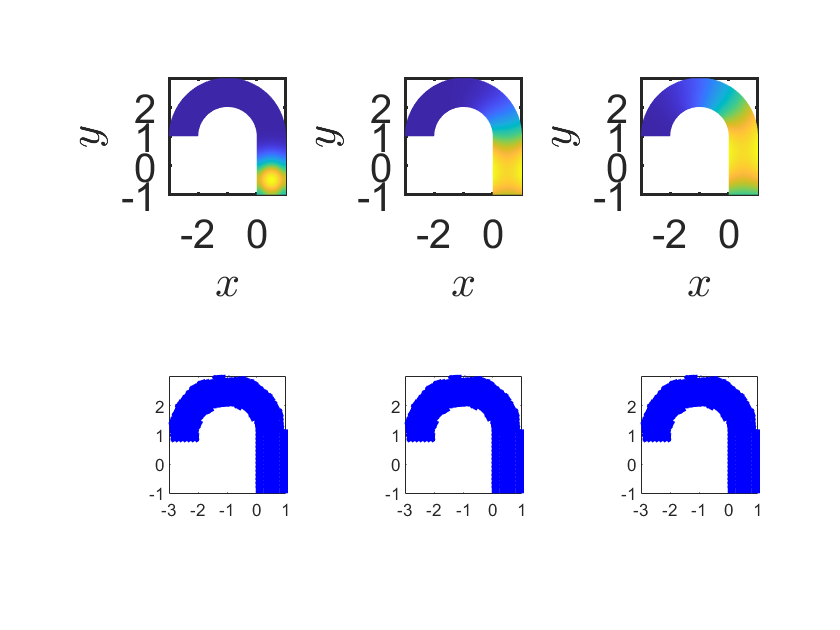
\includegraphics[scale=0.7]{Test101FW.png}
    	\caption{Test1 Forward $\kappa = 1$, $t =1, 10, 19, n = 20$} 
    	\label{FTest11FW}
    \end{figure}
    \begin{figure}[h]
    	\centering
    	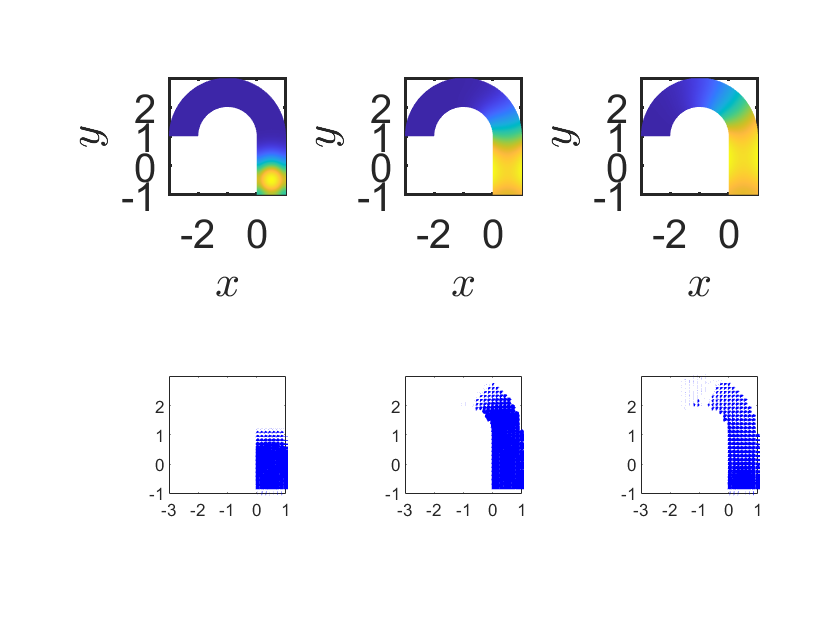
\includegraphics[scale=0.7]{Test101Opt.png}
    	\caption{Test1 Optimization $\kappa = 1$ $t =1, 10, 19, n = 20$} 
    	\label{FTest11Opt}
    \end{figure}
    
    \subsection{Example 2}
    We choose the initial condition for $\rho$ to be $exp(-2((y1 - 0.5 )^2 + (y2 + 0.5)^2))$ and solve a forward problem with constant velocity of strength five, see Figure \ref{FTest2FW}.
    \begin{figure}[h]
    	\centering
    	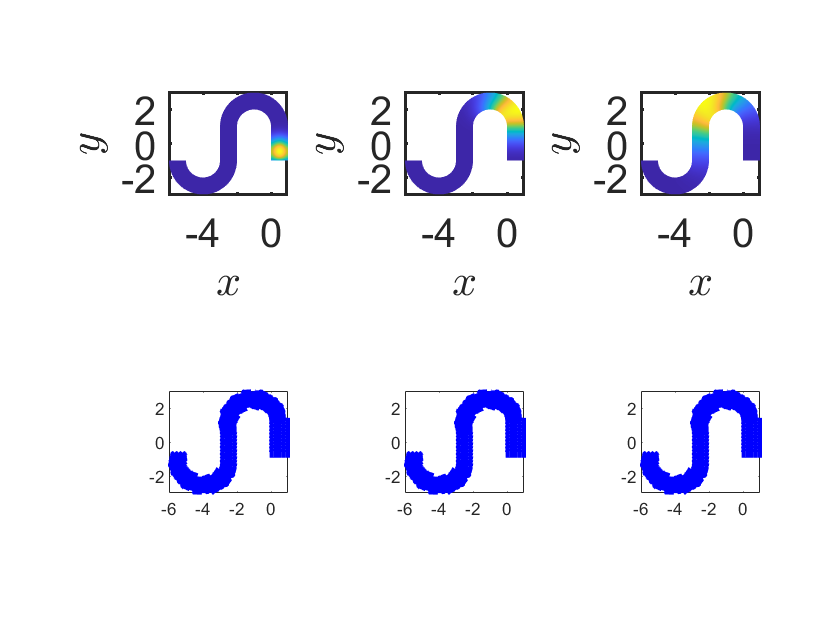
\includegraphics[scale=0.7]{Test11FW.png}
    	\caption{Test2 Forward $t =1, 10, 19, n = 20$} 
    	\label{FTest2FW}
    \end{figure}
    Then we use this forward solution as a target in the OCP, with initial velocity zero. We set $\beta = 10^{-3}$, we solve with tolerances $10^{-7}/ 10^{-3}$, because of time constraints, and $n = 20$, $N = 20$. The solution can be seen in Figure \ref{FTest2Opt}. Again, as expected, the control follows the particle mass. It takes $ 587$ iterations, but the time it takes is $ 5 \times 10^4$. We get $J_{FW} =  0.1921$, $J_{Opt} =  0.0326$. Figures \ref{FTest2Optk1} and \ref{FTest2Optn1} show the results for different interactions. 
    \begin{figure}[h]
    	\centering
    	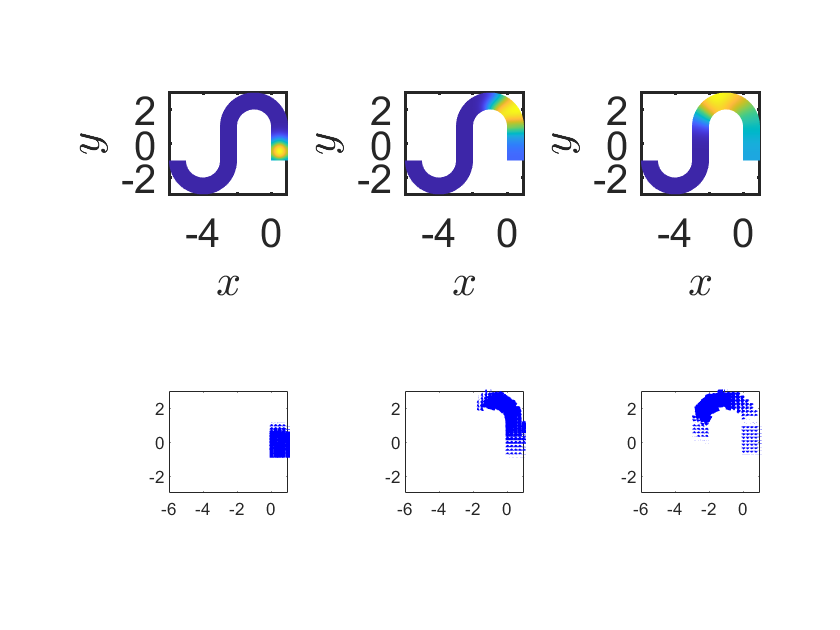
\includegraphics[scale=0.7]{Test11Opt.png}
    	\caption{Test2 Optimization $\kappa = 0$, $t =1, 10, 19, n = 20$} 
    	\label{FTest2Opt}
    \end{figure}
    
    
    \begin{figure}[h]
    	\centering
    	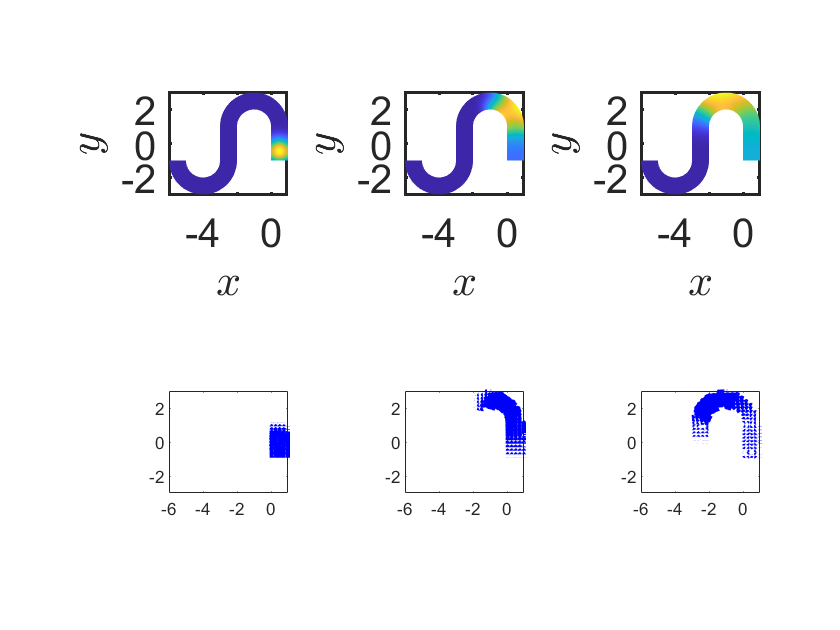
\includegraphics[scale=0.7]{Test11Optk1.png}
    	\caption{Test2 Optimization $\kappa = 1$, $t =1, 10, 19, n = 20$} 
    	\label{FTest2Optk1}
    \end{figure}
\begin{figure}[h]
	\centering
	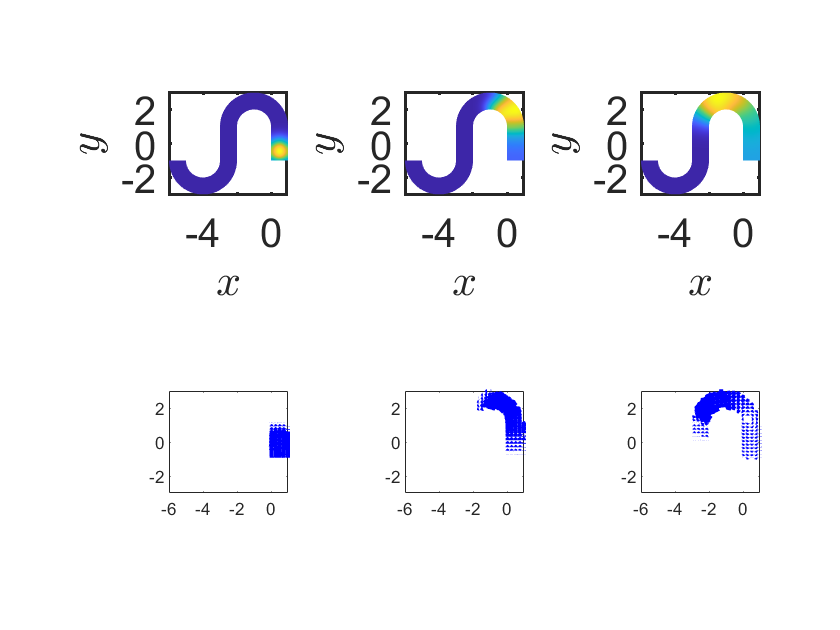
\includegraphics[scale=0.7]{Test11Optn1.png}
	\caption{Test2 Optimization $\kappa = -1$, $t =1, 10, 19, n = 20$} 
	\label{FTest2Optn1}
\end{figure}
    
    \section{Things that do not work}
    1. Giving the forward problem with the constant velocity as initial guess AND as target for the OCP and ask it to do better. It immediately diverges. Maybe too advection dominant?\\
    2. Considering problem 2 above with velocity strength 10 and interaction term. Diverges. Advection dominance?\\
    3. In and outflow BCs. Diverges immediately. Correct implementation? Or maybe this restricts too much and we can't actually change the flow much...  
    
    \section{This Week}
    Regarding the things that do not work:
    1. Probably a bad initial guess.
    2. Instead of higher velocity, we run the problem for longer times. This seems to work (at least for the first few iteration) but it's running on the server at the moment/ the server is down so it might not be. Each iteration takes appropriately longer.
    3. We said that $w=0$ may not be a good initial guess, but $w = 1$ may be. It isn't it diverges too very quickly. We also said that this is probably a very hard OCP to solve (even without MultiShape), so we need more investigation there -- maybe on a box. Ben said to park this problem for now.
    However, what about source control or inflow control. Is it worth writing down an inflow control problem maybe?
    
    \section{Time}
    The problems on multishape take more time than the problems without. Tested AdvectionDiffusion Flow Control Exact problem on a box with $N = 30$, $n = 20$. This takes $36$ seconds with multishape and $9$ seconds for the standard box. Maybe I am measuring wrong but I don't think so.
    When doing the same with $N = 20$, $n = 20$ we get that the MultiShape box solves in $4$ seconds and the standard Box in $1.6$ seconds. 
    When splitting the box into two parts and evaluate each 'subbox' with $N = 20$, $n = 20$, this solves in $25$ seconds. This is faster than the 'whole' box with $N = 30$, which I think is slightly odd. But not sure. 
    \\
    \\
    I incorporated a count in the code now to evaluate how long each iteration takes (instead of just total time). Since then I haven't run a long OCP to the end, but the first few hundred iterations take each roughly the same amount of time.
    For the two problems above this is on average $20$ seconds per iteration.
    The fancy channel (see Figure \ref{FFCFW} for target) however takes $180$ seconds per iteration, which is why I had to stop it on my machine after $250$ iterations. It converged to almost $10^{-2}$ in that time though so I am reasonably confident that this works. The target is a background flow of strength one, and diffusion.
    \begin{figure}[h]
    	\centering
    	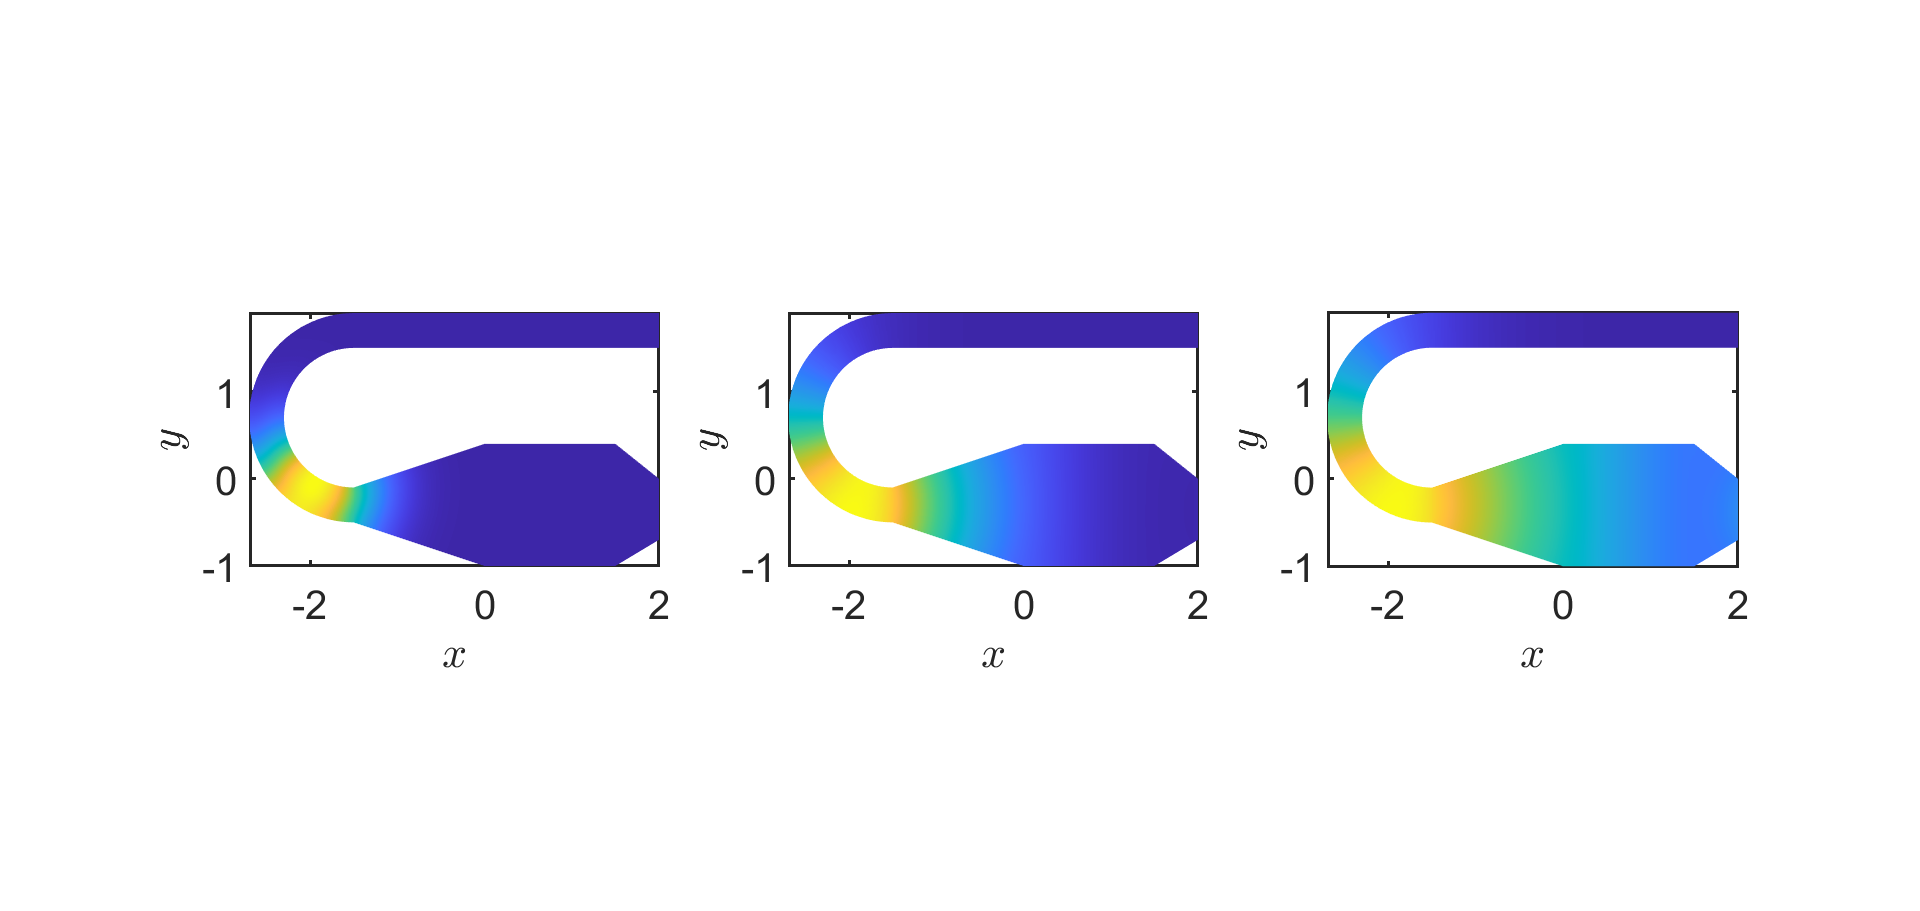
\includegraphics[scale=0.3]{FancyChannelFW.png}
    	\caption{Fancy Channel Target} 
    	\label{FFCFW}
    \end{figure}
    \section{Time savings}
    We talked about a few things that I can do to make the code quicker.
    The first one is to solve a problem on a sparse grid, interpolate the solution onto a fine grid and run it again, hoping the IG from the sparse grid will make convergence faster.
    This will probably work, but I am currently stuck at the interpolation matrix. It is 'loosing points'.
    \\
    The second idea is to take the solution for $\kappa = 0$ to solve for $\kappa = 1$, $\kappa = -1$. This is because the solutions for the three interaction strengths are not as different from each other as they are from $w = 0$. 
    I have tried this for $\kappa = 1$. This converges in $347$ iteration, which is a saving of $104$ iterations compared to starting with $w = 0$. Each iteration takes around $20$ seconds, but since I was doing other things on my laptop, resulting in iterations that took much longer, this averages to $22.5$ seconds per iteration.\\
    Another thing to do is to datastore the multishape itself but I have issues with this at the moment.\\
    Another thing is to do an adaptive $\lambda$, but haven't tried that yet because if you get it wrong, you need to start at the beginning and that takes hours.
       
    \section{Other}
    I had some issues with matlab having memory issues and it is showing on the task manager too that at times it uses literally all of my laptops memory. Why? A lot of recovering results from datastorage? What can be done?
    
    \section{Classes}
    How to enrol in Introduction to Optimization as listener only.\\
    How do I enrol in School of Informatics classes?\\
    Do we know when the Python class starts?\\
    Should I take the MAC-MIGS course for credits or something else (given that we said I should get my credits done in semester 1).
       
    
\end{document}